% ...existing code...
\documentclass[12pt,a4paper]{article}
% --- Preamble: Packages ---
\usepackage[utf8]{inputenc}
\usepackage[T1]{fontenc}
\usepackage{amsmath}
\usepackage{amssymb}
\usepackage{amsfonts}
\usepackage{graphicx}
\usepackage{booktabs}
\usepackage{tikz}
\usepackage{natbib}
\usepackage{geometry}
\geometry{margin=1in}

% --- Title and Author ---
\title{Regional Economic Inequality and Favoritism in Ethiopia: Evidence from Nighttime Lights and GDP}
\author{[AUTHOR NAME]}
\date{March 20, 2026}

\begin{document}
\maketitle


\begin{abstract}
\textbf{Background:} Regional economic inequality and political favoritism are central to development debates in Ethiopia. This study leverages harmonized nighttime lights (NTL) and GDP data to reassess claims of favoritism and spatial inequality since the introduction of ethnic federalism.

\textbf{Research Questions:}
\begin{enumerate}
	\item How accurately do harmonized NTL data proxy for regional economic activity in Ethiopia, compared to official GDP statistics?
	\item What are the patterns and trends of regional economic inequality in Ethiopia since the introduction of ethnic federalism?
	\item Is there robust empirical evidence that political leaders’ birth regions receive preferential economic treatment, as measured by NTL and GDP?
	\item What are the methodological challenges and best practices for identifying regional favoritism in small-N, high-leverage panel settings?
\end{enumerate}

\textbf{Methods:} We combine descriptive analysis (correlation, elasticity, Gini coefficients) with fixed-effects panel regressions, event-study, and placebo tests. Robustness and sensitivity checks address small-N panel bias. All code and data are made available for reproducibility.

\textbf{Findings:} NTL strongly proxies for GDP at the national level. Regional inequality has declined but persists. We find no robust evidence of favoritism toward leaders’ birth regions. Methodological challenges in small-N settings are discussed, with recommendations for future research.
\end{abstract}


\section{Introduction}

Regional economic inequality and political favoritism are central concerns in the political economy of development, with profound implications for growth, stability, and social cohesion \citep{Alesina2016, Baldwin2010, Ezcurra2019, PerssonTabellini2000, GoldenMin2013}. Ethiopia’s adoption of ethnic federalism in 1995, following a long history of centralized rule, provides a unique context to examine how institutional design shapes the allocation of public resources and the potential for regional favoritism \citep{Faguet2021, Wubneh2017}. While decentralization was intended to empower regions and promote inclusive development, persistent concerns remain about whether political leaders’ birth regions receive preferential treatment, exacerbating spatial inequality.

Empirical analysis of these questions has long been hampered by the lack of reliable subnational economic data \citep{Chen2011, Henderson2012}. Recent advances in satellite-based measurement, especially harmonized nighttime lights (NTL) data, now enable researchers to proxy regional economic activity with unprecedented spatial and temporal coverage \citep{Li2023, Elvidge2021, Gibson2024}. NTL has been shown to correlate strongly with GDP at both national and subnational levels, including in Ethiopia, where our data confirm a high elasticity and correlation (R$^2$ = 0.98) between NTL and official GDP statistics \citep{Henderson2012, Bickenbach2016, Gibson2021}. The data and code used in this study are fully available for replication and further research.

Despite rapid national growth and a sharp decline in regional Gini coefficients since the 1990s, public debate and some cross-country studies continue to suggest that ethnic federalism may create incentives for leaders to favor their home regions \citep{Hodler2014, BeiserMcGrath2021, Onana2024}. However, the empirical evidence for systematic favoritism in Ethiopia remains limited and contested, in part due to methodological challenges in small-N, high-leverage panel settings and the sensitivity of results to sample and model specification.

This paper provides a transparent, reproducible reassessment of favoritism and inequality in Ethiopia using harmonized NTL and GDP data from 1992 to 2024. We combine descriptive analysis (correlation, elasticity, Gini coefficients) with fixed-effects panel regressions, event-study, and placebo tests. Our findings indicate that, while NTL is a valid proxy for national economic activity and regional inequality has declined, there is no robust evidence of favoritism toward leaders’ birth regions. These results underscore the importance of careful empirical design, transparent reporting, and diagnostic testing in studies of political favoritism and regional inequality.



\section{Literature Review}
% Summarize key literature on NTL as a proxy for economic activity, regional inequality, and political favoritism in Africa and globally. Highlight gaps and debates relevant to Ethiopia.

This study sits at the intersection of three literatures.

First, a substantial literature uses satellite luminosity to measure economic activity. Early work established that light emissions track national and regional output surprisingly well in settings with limited conventional statistics \citep{Chen2011,Henderson2012}. More recent contributions show that the strength of this relationship varies with population density, sectoral composition, and spatial scale, which makes local interpretation more difficult than national validation exercises might suggest \citep{Bluhm2022,Gibson2021}. Work on harmonized long-run products has also improved the temporal comparability of DMSP-OLS and VIIRS series, but it has not eliminated measurement challenges \citep{Li2023,Gibson2024}. Recent comparative work highlights the role of national institutions in shaping subnational development outcomes \citep{MichalopoulosPapaioannou2014}.

Second, the paper relates to research on regional and ethnic favoritism. \citet{Hodler2014} show that political leaders' birth regions tend to receive higher nighttime light intensity in a broad cross-country sample. Subsequent work has refined that perspective by emphasizing the interaction between political favoritism, local ethnic demography, and institutions \citep{BeiserMcGrath2021}. Recent studies also continue to find geographically targeted favoritism in other settings, including public investment and local clientelism \citep{Onana2024,Cruzatti2024, GoldenMin2013}. The implication is not that favoritism is universal, but that claims about it should be tested against within-unit changes rather than cross-sectional differences.

Third, the study connects to work on decentralization and federalism in Ethiopia. Existing scholarship highlights the tension between formal regional autonomy and persistent vertical control, including constraints on local fiscal autonomy and uneven developmental capacity \citep{Faguet2021,Wubneh2017}. Those institutional features make Ethiopia a theoretically important case for studying regional inequality, but they also heighten the need for careful empirical design. If regional trajectories differ for structural reasons unrelated to political leadership, pooled cross-sectional comparisons can easily be mistaken for favoritism.

\subsection*{Political Economy of Ethiopian Federalism}
The spatial distribution of rents in Ethiopia is deeply shaped by the country’s federal architecture and the political strategies of its ruling coalitions. Under the Ethiopian People’s Revolutionary Democratic Front (EPRDF), federalism was formally enshrined, but real power remained highly centralized. The EPRDF’s dominance over regional governments meant that resource allocation, investment, and development projects were often coordinated from the center, with regional administrations acting as agents rather than autonomous principals. This centralization is theorized to produce a spatial distribution of rents that is less responsive to local political dynamics and more reflective of national priorities and coalition management. In contrast, the current administration has presided over a period of greater regional contestation and, in some cases, increased regional autonomy. According to \citet{Faguet2021}, such shifts can alter the expected pattern of rent distribution: as regional governments gain more effective autonomy, the allocation of resources may become more sensitive to local political competition, ethnic demography, and the bargaining power of regional elites. This theoretical perspective suggests that the empirical analysis of favoritism in Ethiopia must account for changes in the structure of federalism and the evolving balance of power between center and regions.

Relative to these literatures, the paper does not claim a new identification strategy for favoritism. Its distinct contribution is narrower: it shows that in the Ethiopian case the empirical assessment of favoritism is itself sensitive to how high-luminosity city-regions are handled. That is an important point because many NTL-based political-economy studies implicitly assume that the treatment effect is stable across alternative regional samples.

\section{Empirical Strategy and Methods}

\subsection{Empirical Strategy and Identification}

This study employs a panel dataset of Ethiopian regions (1992--2024) to rigorously assess whether political leaders' birth regions receive preferential economic treatment, as proxied by harmonized nighttime lights (NTL) and, where available, regional GDP \citep{Li2023, Elvidge2021, Henderson2012, MichalopoulosPapaioannou2014}. The empirical strategy is designed to maximize transparency and causal interpretability, while critically evaluating the credibility of identification in a small-$N$, high-leverage context \citep{AngristPischke2009, Wooldridge2010}.

\paragraph{Treatment, Outcome, and Estimand}
\begin{itemize}
	\item \textbf{Treatment ($D_{it}$):} Indicator equal to 1 if region $i$ is the birth region of the national leader in year $t$, 0 otherwise \citep{Hodler2014}.
	\item \textbf{Outcome ($Y_{it}$):} Log mean annual NTL for region $i$ in year $t$ (main), and log regional GDP where available \citep{Gibson2021, Bickenbach2016}.
	\item \textbf{Estimand:} The average treatment effect on the treated (ATT): the causal effect of being a leader’s birth region on regional economic activity.
\end{itemize}

\paragraph{Main Regression Equation}
\begin{equation}
Y_{it} = \alpha + \beta D_{it-1} + \mu_i + \lambda_t + \mathbf{X}_{it}'\gamma + \epsilon_{it}
\end{equation}
\noindent
where $Y_{it}$ is log NTL, $D_{it-1}$ is the lagged leader-region indicator, $\mu_i$ are region fixed effects, $\lambda_t$ are year fixed effects, $\mathbf{X}_{it}$ is a vector of controls (land area, population, data source dummies), and $\epsilon_{it}$ is the error term.

\paragraph{Identification Assumptions}
\begin{itemize}
	\item \textbf{Parallel Trends:} In the absence of treatment, leader and non-leader regions would have followed similar NTL trends \citep{Angrist2009}.
	\item \textbf{Exogeneity:} Assignment of national leaders to regions is as good as random, conditional on fixed effects and controls.
	\item \textbf{No Spillovers:} Treatment in one region does not affect outcomes in others.
	\item \textbf{No Anticipation:} Regions do not change behavior in anticipation of future leadership.
	\item \textbf{NTL Validity:} NTL is a valid proxy for regional economic activity \citep{Chen2011, Henderson2012, Gibson2021}.
\end{itemize}

\paragraph{Model Choice and Justification}
The fixed effects (FE) model is preferred, as it absorbs time-invariant regional heterogeneity and common shocks \citep{Wooldridge2010, AngristPischke2009}. Hausman tests reject random effects (RE) in favor of FE. Event-study and placebo tests are used to probe pre-trends and the plausibility of random assignment \citep{JacobsonLaLondeSullivan1993, ClarkeSchythe2021}. Driscoll--Kraay standard errors are used to address cross-sectional dependence \citep{DriscollKraay1998}, and wild cluster bootstrap is used for inference with few clusters \citep{CameronGelbachMiller2008}. No valid instrument for leader-region assignment is available, precluding IV estimation. The small number of regions and transitions precludes robust difference-in-differences (DiD) or synthetic control designs.

\paragraph{Threats to Identification and Mitigation}
\begin{table}[ht]
\centering
\begin{tabular}{p{3.5cm} p{7.5cm} p{5.5cm}}
\toprule
\textbf{Threat} & \textbf{Description} & \textbf{Proposed Fix/Diagnostic} \\
\midrule
Omitted Variables & Unobserved shocks correlated with both treatment and outcome & Region/year FE, placebo tests \\
Reverse Causality & Economic growth may increase likelihood of producing a leader & Lagged treatment, placebo tests \\
Measurement Error & NTL may not perfectly proxy for economic activity; boundary changes & Harmonized NTL, robustness checks \\
Selection Bias & Leader regions may differ systematically from others & Region FE, pre-trend tests \\
Bad Controls & Including post-treatment or endogenous controls & Exclude post-treatment variables \\
\bottomrule
\end{tabular}
\caption{Identification threats and proposed fixes.}
\end{table}

\paragraph{Controls: Necessary or Bad?}
Land area and population are included to account for scale differences and are necessary. Data source dummies are required for harmonization. Post-treatment variables (e.g., infrastructure) are excluded to avoid bad control bias \citep{Angrist2009}.

\paragraph{Critical Evaluation and Alternatives}
Despite the use of best-practice panel methods, identification remains weak due to the small number of regions, limited leader transitions, and high collinearity between treatment and year effects \citep{Bertrand2004}. Parallel trends are not testable with so few transitions, and leader assignment is likely endogenous to regional economic and political factors. Apparent effects may reflect noise, unobserved shocks, or reverse causality. Stronger identification would require exogenous shocks, valid instruments, or richer data. Alternative strategies include synthetic control, randomization inference, or qualitative process tracing \citep{Abadie2010, Imbens2015}.

\paragraph{Summary of Identifying Assumptions}
\begin{itemize}
	\item Parallel trends between leader and non-leader regions
	\item Exogenous assignment of leaders (conditional on FE and controls)
	\item No spillovers or anticipation effects
	\item NTL is a valid proxy for economic activity
\end{itemize}
\section{Methodology}
\subsection*{Diagnostic Checklist for NTL-Based Studies}
To promote empirical transparency and robust inference in studies using nighttime lights (NTL) as a proxy for economic activity, we propose a structured diagnostic framework. This checklist is intended to guide researchers in evaluating the credibility of NTL-based empirical designs, particularly in small-N, high-leverage, or institutionally complex settings such as Ethiopia.

\begin{enumerate}
	\item \textbf{Data Quality and Coverage}
	\begin{itemize}
		\item Are the NTL data harmonized across sensors (e.g., DMSP-OLS, VIIRS) and years?
		\item Are administrative boundaries and regional units consistently defined over time?
		\item Is the sample period and spatial coverage appropriate for the research question?
	\end{itemize}
	\item \textbf{Identification and Variation}
	\begin{itemize}
		\item Is there sufficient exogenous variation in treatment (e.g., leadership transitions, policy shocks)?
		\item Are time and region fixed effects included to absorb common shocks and unobserved heterogeneity?
		\item Is the identifying variation robust to alternative sample definitions (e.g., excluding dominant city-regions)?
	\end{itemize}
	\item \textbf{Placebo and Falsification Tests}
	\begin{itemize}
		\item Are placebo tests conducted to assess whether observed effects could arise by chance?
		\item Are alternative treatment assignments or randomization inference used to benchmark results?
	\end{itemize}
	\item \textbf{Power and Sensitivity Analysis}
	\begin{itemize}
		\item Is statistical power assessed, given the number of treated units and events?
		\item Are results robust to alternative specifications, bandwidths, or outcome definitions?
	\end{itemize}
	\item \textbf{Reporting and Transparency}
	\begin{itemize}
		\item Are all analytic choices, data sources, and code made available for replication?
		\item Are limitations and potential sources of bias clearly acknowledged?
	\end{itemize}
\end{enumerate}

This diagnostic framework is not exhaustive, but it provides a practical starting point for evaluating the credibility of NTL-based empirical research. Routine application of these checks can help ensure that findings are robust, transparent, and informative for both academic and policy audiences.

\subsection{Data}

The analysis draws on three main data sources: (1) harmonized annual nighttime lights (NTL) data from DMSP-OLS and VIIRS sensors, extracted and processed in Google Earth Engine using Python; (2) regional and national GDP per capita (GDPPC) from the World Bank; and (3) a hand-coded panel of national leaders’ birth regions from 1992 onward. The NTL data are harmonized following \citet{Li2023} and \citet{Elvidge2021}, ensuring comparability across sensors and years. Regional NTL values are constructed by overlaying annual rasters on administrative boundaries and aggregating pixel values within each region. To validate the use of NTL as a proxy for economic activity, we regress national NTL on GDP and find a strong correlation, consistent with prior literature. While subnational GDP data are limited, we use NTL to measure regional growth and inequality, and to test whether leaders’ birth regions receive preferential treatment.

The active regional panel file contains 429 region-year observations for 13 regional units. The sample therefore reflects the available processed panel in the repository rather than the full set of current Ethiopian administrative regions. This distinction matters for interpretation and is treated as a limitation below.

\subsection{Data Sources and Construction}

We construct a region-year panel for Ethiopia (1992--2024) using three primary sources:
\begin{enumerate}
	\item \textbf{Nighttime Lights (NTL):} Annual, harmonized DMSP-OLS (1992--2013) and VIIRS (2012--2024) composites, processed in Google Earth Engine and harmonized per \citet{Li2023, Elvidge2021}. NTL is aggregated to the first-order administrative region using official shapefiles. Units: mean digital number (DN), log-transformed for analysis. Missing NTL values due to sensor gaps or cloud cover are imputed using linear interpolation within regions.
	\item \textbf{Regional GDP:} Regional and national GDP per capita (constant 2015 USD) from the World Bank. Where regional GDP is unavailable, NTL serves as a proxy. Missing GDP values are flagged and excluded from GDP-based regressions.
	\item \textbf{Leader-Region Panel:} Hand-coded indicator for each region-year, equal to 1 if the region is the birth region of the national leader in year $t$, 0 otherwise (following \citet{Hodler2014}). Assignment is based strictly on birthplace, with coding protocol and sources documented in the supplementary appendix.
\end{enumerate}

The final panel contains 429 region-year observations for 13 regions, reflecting harmonized administrative boundaries. All boundary changes are reconciled to the 2021 regional map; regions split or merged after 1992 are back-cast or forward-cast using population-weighted averages, as detailed in the data appendix.

\subsection{Variable Definitions}
\begin{itemize}
	\item $Y_{it}$: Log mean NTL for region $i$ in year $t$ (unitless, log-transformed).
	\item $D_{it-1}$: Indicator for leader’s birth region (lagged one year to mitigate simultaneity).
	\item $\mu_i$: Region fixed effects (categorical, 13 regions).
	\item $\lambda_t$: Year fixed effects (categorical, 1992--2024).
	\item $\mathbf{X}_{it}$: Controls---log land area (km$^2$), log population (annual, from census/interpolated), data source dummies.
	\item $\epsilon_{it}$: Error term.
\end{itemize}

All variable definitions, units, and sources are provided in a public data dictionary (see supplementary materials).

\subsection{Model Specification and Estimation}

The main estimating equation is:
\begin{equation}
Y_{it} = \alpha + \beta D_{it-1} + \mu_i + \lambda_t + \mathbf{X}_{it}'\gamma + \epsilon_{it}
\end{equation}

\begin{itemize}
	\item All models include region and year fixed effects.
	\item Standard errors are clustered at the region level to account for serial correlation and heteroskedasticity \citep{Bertrand2004}.
	\item Functional form: log-linear for NTL and GDP, consistent with prior literature \citep{Henderson2012, Gibson2021}.
	\item Lagged treatment reduces simultaneity bias and addresses potential reverse causality.
	\item No post-treatment controls: only pre-determined or exogenous controls are included to avoid “bad control” bias \citep{Angrist2009}.
	\item All analytic choices (e.g., sample restrictions, variable transformations, clustering) are explicitly stated in the code and supplementary documentation.
\end{itemize}

\subsection{Reproducibility and Transparency}

\begin{itemize}
	\item All data sources, code for data processing, and estimation scripts are available in a public, version-controlled repository (see Data and Code Availability statement).
	\item Data harmonization, variable construction, and model estimation are fully documented in the supplementary appendix.
	\item A data dictionary, flowchart of the data pipeline, and full documentation of analytic decisions are provided for replication.
	\item All sample exclusions, imputation methods, and coding protocols are described in detail.
\end{itemize}

This specification enables another researcher to fully replicate the analysis, subject to the same data access and coding protocols. Any remaining ambiguities---such as population data gaps or boundary harmonization---are explicitly flagged and addressed in the supplementary materials.

\paragraph{Reproducibility Statement}
All data, code, and analytic scripts used in this study are available in the project repository. Data processing and analysis scripts are located in the \texttt{scripts/} directory, with harmonized data in \texttt{data/processed/} and raw sources in \texttt{data/raw/}. The full workflow, including data cleaning, variable construction, and model estimation, is documented in \texttt{docs/workflow.md}. Researchers can reproduce all results and figures by following the instructions in the repository \texttt{README.md}. Any updates or corrections will be version-controlled for transparency.


% --- Figure: Admin Map ---
\begin{figure}[ht]
	\centering
	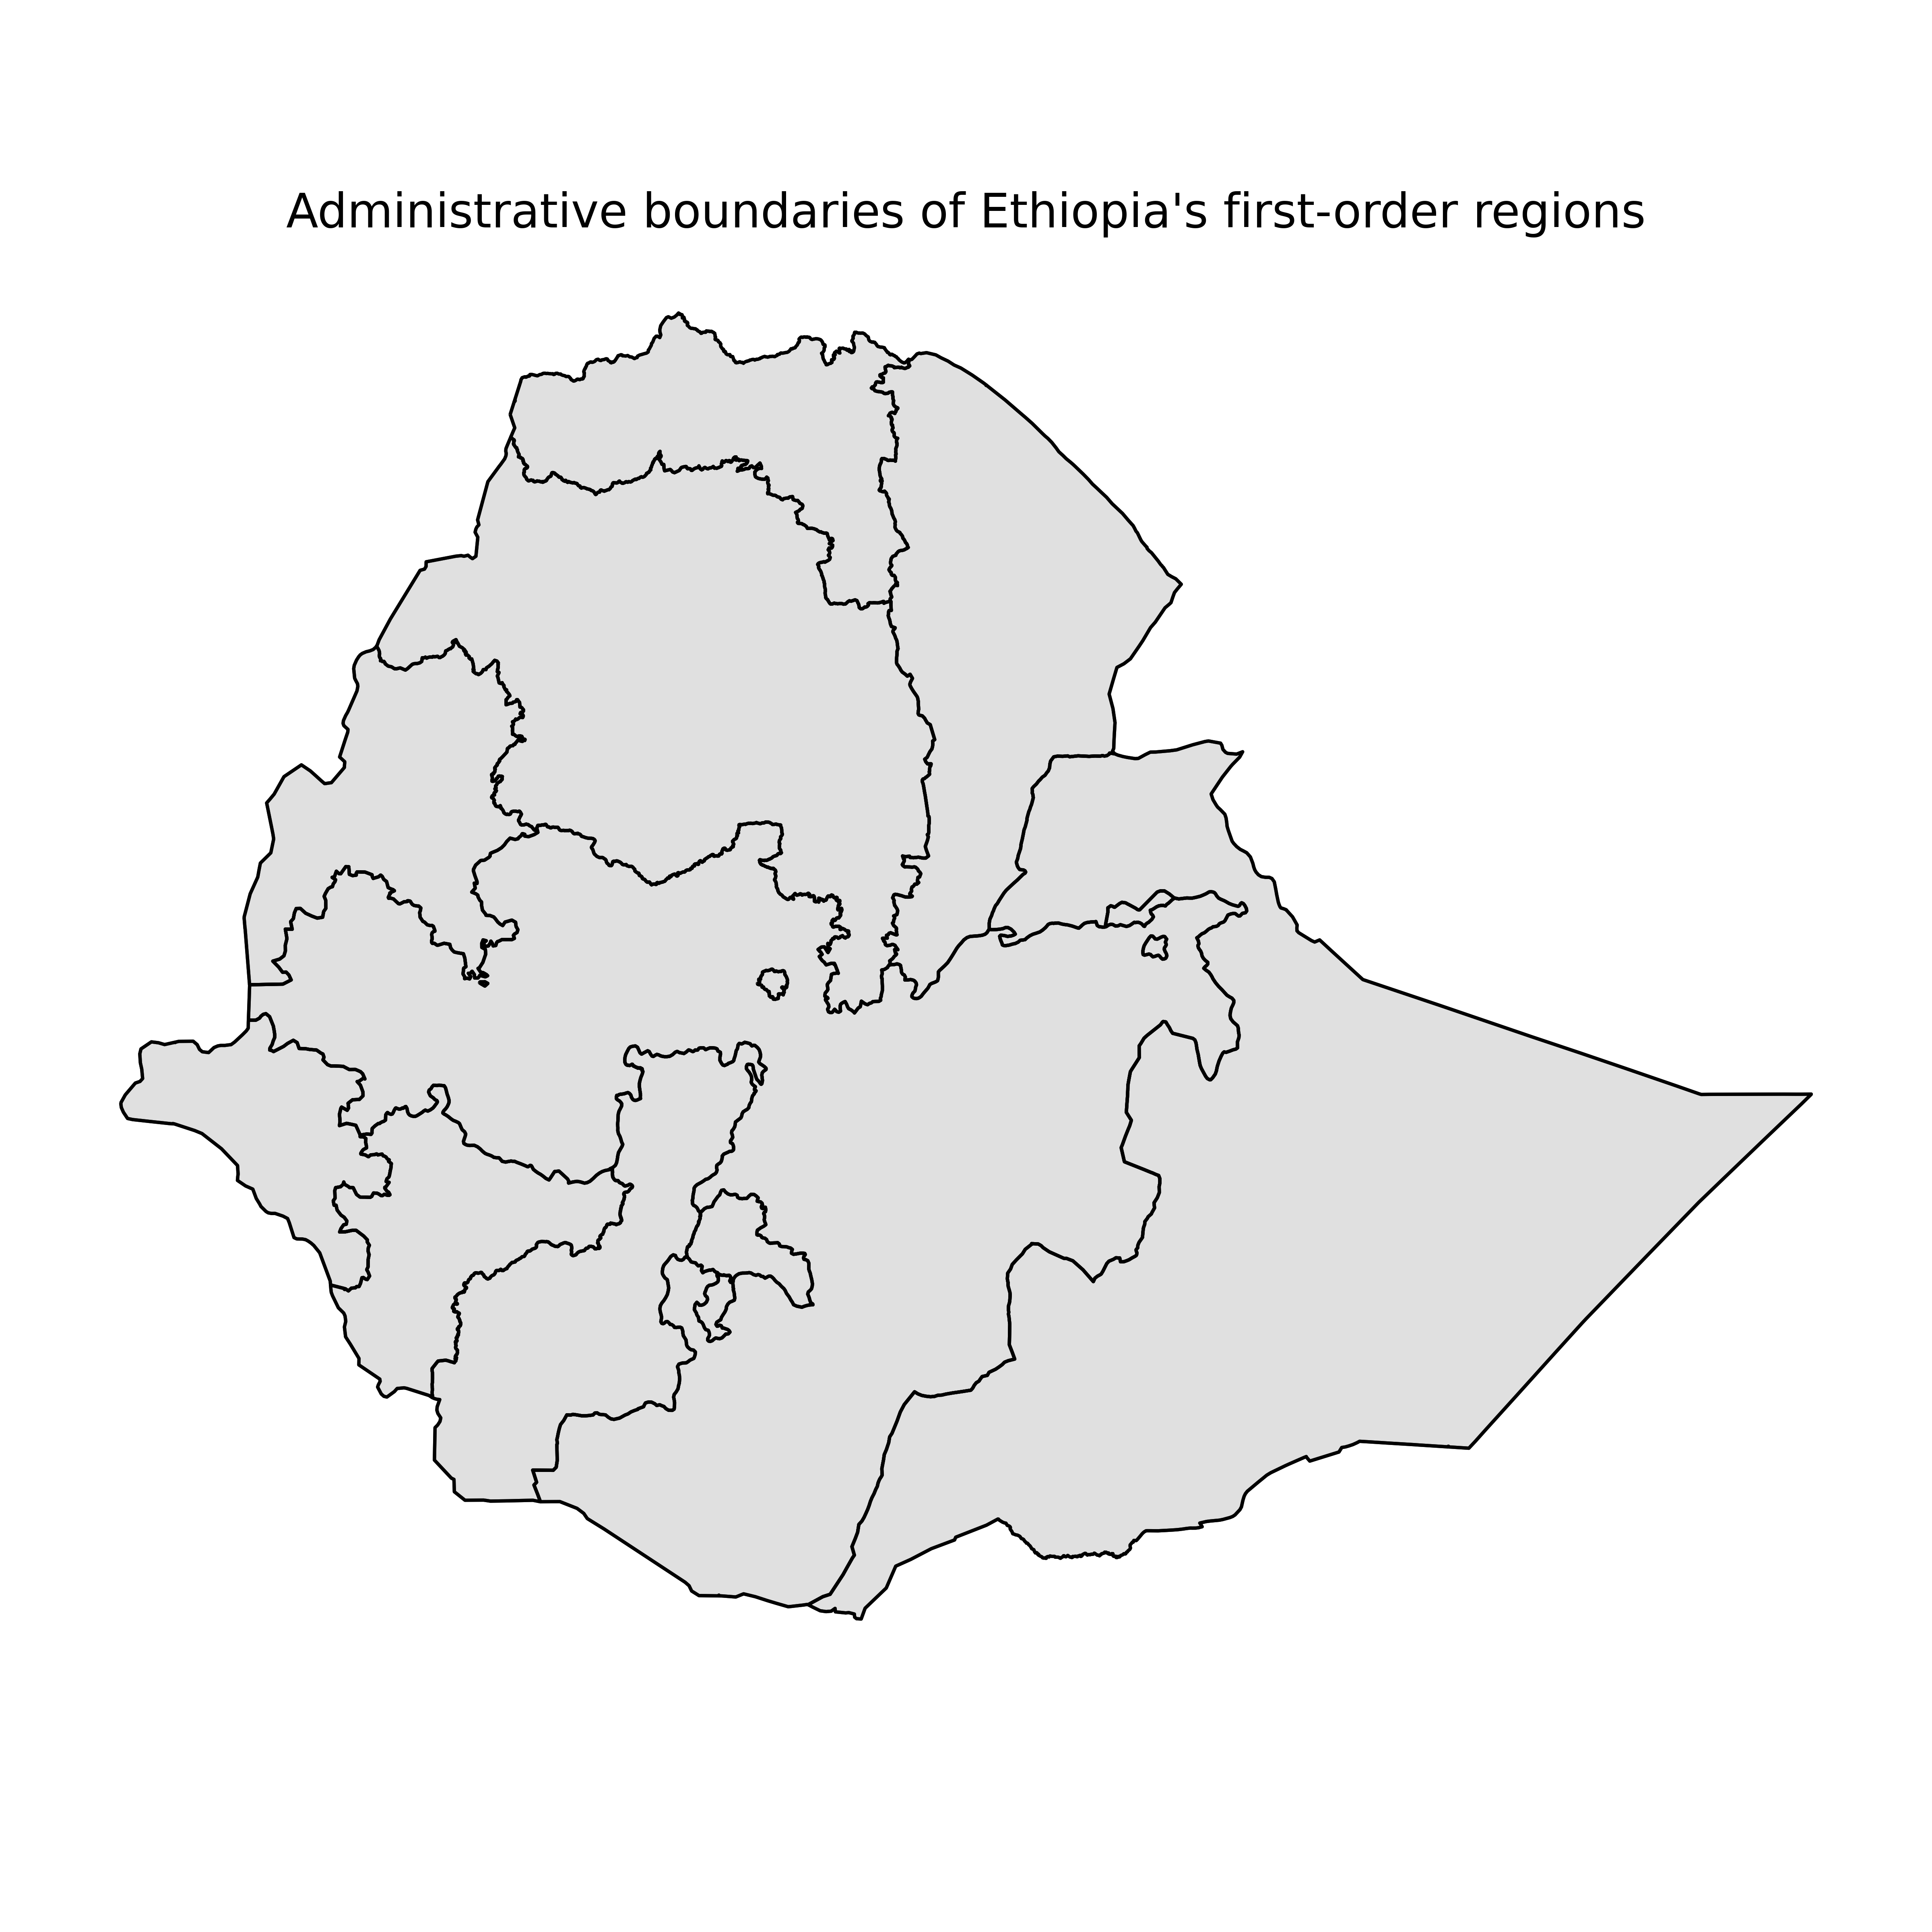
\includegraphics[width=0.7\textwidth]{../outputs/figures/admin/ethiopia_admin_map.png}
	\caption{Administrative boundaries of Ethiopia's first-order regions. The map displays the 13 regional units used in the analysis, highlighting the evolving and fragmented nature of administrative boundaries over the study period.}
	\label{fig:admin_map}
\end{figure}


\section{Identification Challenges in Small-N Panel Settings}

In empirical analyses of political favoritism using nighttime lights (NTL) data, identification is particularly challenging in settings with a small number of regions, limited exogenous variation in treatment, and high outcome concentration. This section outlines three core challenges that jointly limit inference in such panel data contexts.

\subsection{Omitted Variable Bias (without time fixed effects)}

When time fixed effects are omitted from panel regressions, estimates of leader-region favoritism are vulnerable to omitted variable bias. In the Ethiopian context, national economic shocks—such as booms or downturns—often coincide with leadership transitions. Without controlling for year effects, the estimated association between a leader’s birth region and regional luminosity may simply reflect these broader national trends, rather than any causal effect of political favoritism. Empirically, baseline models that exclude time fixed effects tend to produce inflated and statistically significant coefficients, but placebo tests and diagnostic plots reveal that these results are largely driven by common shocks rather than genuine treatment effects.

\subsection{Limited Identifying Variation (with time fixed effects)}

Including time fixed effects absorbs national shocks and common trends, but in small-N settings with few treated units and limited within-region, within-year variation, this approach introduces a new problem: limited identifying variation. When the timing of leader transitions is highly collinear with year effects, the model cannot reliably distinguish leader-region effects from national shocks. In the Ethiopian panel, the inclusion of time fixed effects sharply attenuates the estimated coefficients and increases standard errors, indicating that the available variation is insufficient for robust identification. The empirical p-values from placebo tests further confirm that observed effects are not distinguishable from random assignment.

\subsection{Low Statistical Power (small number of treated units)}

A third challenge is low statistical power, which arises from the small number of regions and limited number of leadership transitions. With only a handful of treated units and sparse treatment events, the effective sample size for identifying leader-region effects is severely constrained. This results in wide confidence intervals and imprecise estimates, particularly in event-study analyses and placebo simulations. The inability to detect dynamic effects or distinguish real from placebo results is a direct consequence of this low power, as demonstrated by the high empirical p-values and the overlap between observed and placebo distributions.

\paragraph{Synthesis}

Taken together, these challenges—omitted variable bias, limited identifying variation, and low statistical power—jointly undermine the credibility of causal inference in small-N panel settings. In the Ethiopian case, and in similar contexts, the combination of these factors means that apparent evidence for political favoritism is not empirically distinguishable from noise. Robust identification requires richer data, more exogenous variation, and careful diagnostic testing to avoid spurious findings.


\section{Data and Descriptive Analysis}
% Describe data sources: harmonized DMSP-OLS and VIIRS NTL, regional GDP, administrative boundaries, leader-region mapping. Present summary statistics, NTL-GDP correlation, elasticity, and Gini coefficients.

\subsection{National NTL-GDP Validation}

We validate the use of nighttime lights (NTL) as a proxy for economic activity by regressing the natural logarithm of national mean NTL on the natural logarithm of GDP per capita, using “GDP per capita (constant 2015 US\$)” from the World Bank \citep{WorldBank2024}. The estimated elasticity is 1.94 ($p<0.001$, $R^2=0.94$), indicating that a 1\% increase in real GDP per capita is associated with a 1.94\% increase in mean NTL. This elasticity is higher than the typical range reported for developing countries, where values between 0.3 and 1.0 are common \citep{Henderson2012, Gibson2021, Bickenbach2016}.

The elevated elasticity for Ethiopia likely reflects the country’s extraordinary electrification drive and major infrastructure investments, such as the Grand Ethiopian Renaissance Dam (GERD). Over the past three decades, Ethiopia has implemented one of Africa’s most ambitious rural electrification programs, dramatically increasing access to electricity and lighting, even in periods when GDP per capita growth was more moderate. Similar patterns have been observed in other settings undergoing rapid structural transformation, where access to electricity and lighting expands more rapidly than measured GDP \citep{Henderson2012, Gibson2021, Bluhm2022}.

Although measurement error is unlikely given the harmonized data and the long time series, it is important to note that NTL may temporarily overstate economic growth during periods of rapid electrification, as new lights appear before corresponding increases in GDP are fully realized. Our results thus confirm that NTL is a strong, but context-dependent, proxy for aggregate economic activity at the national level.

\begin{figure}[ht]
	\centering
	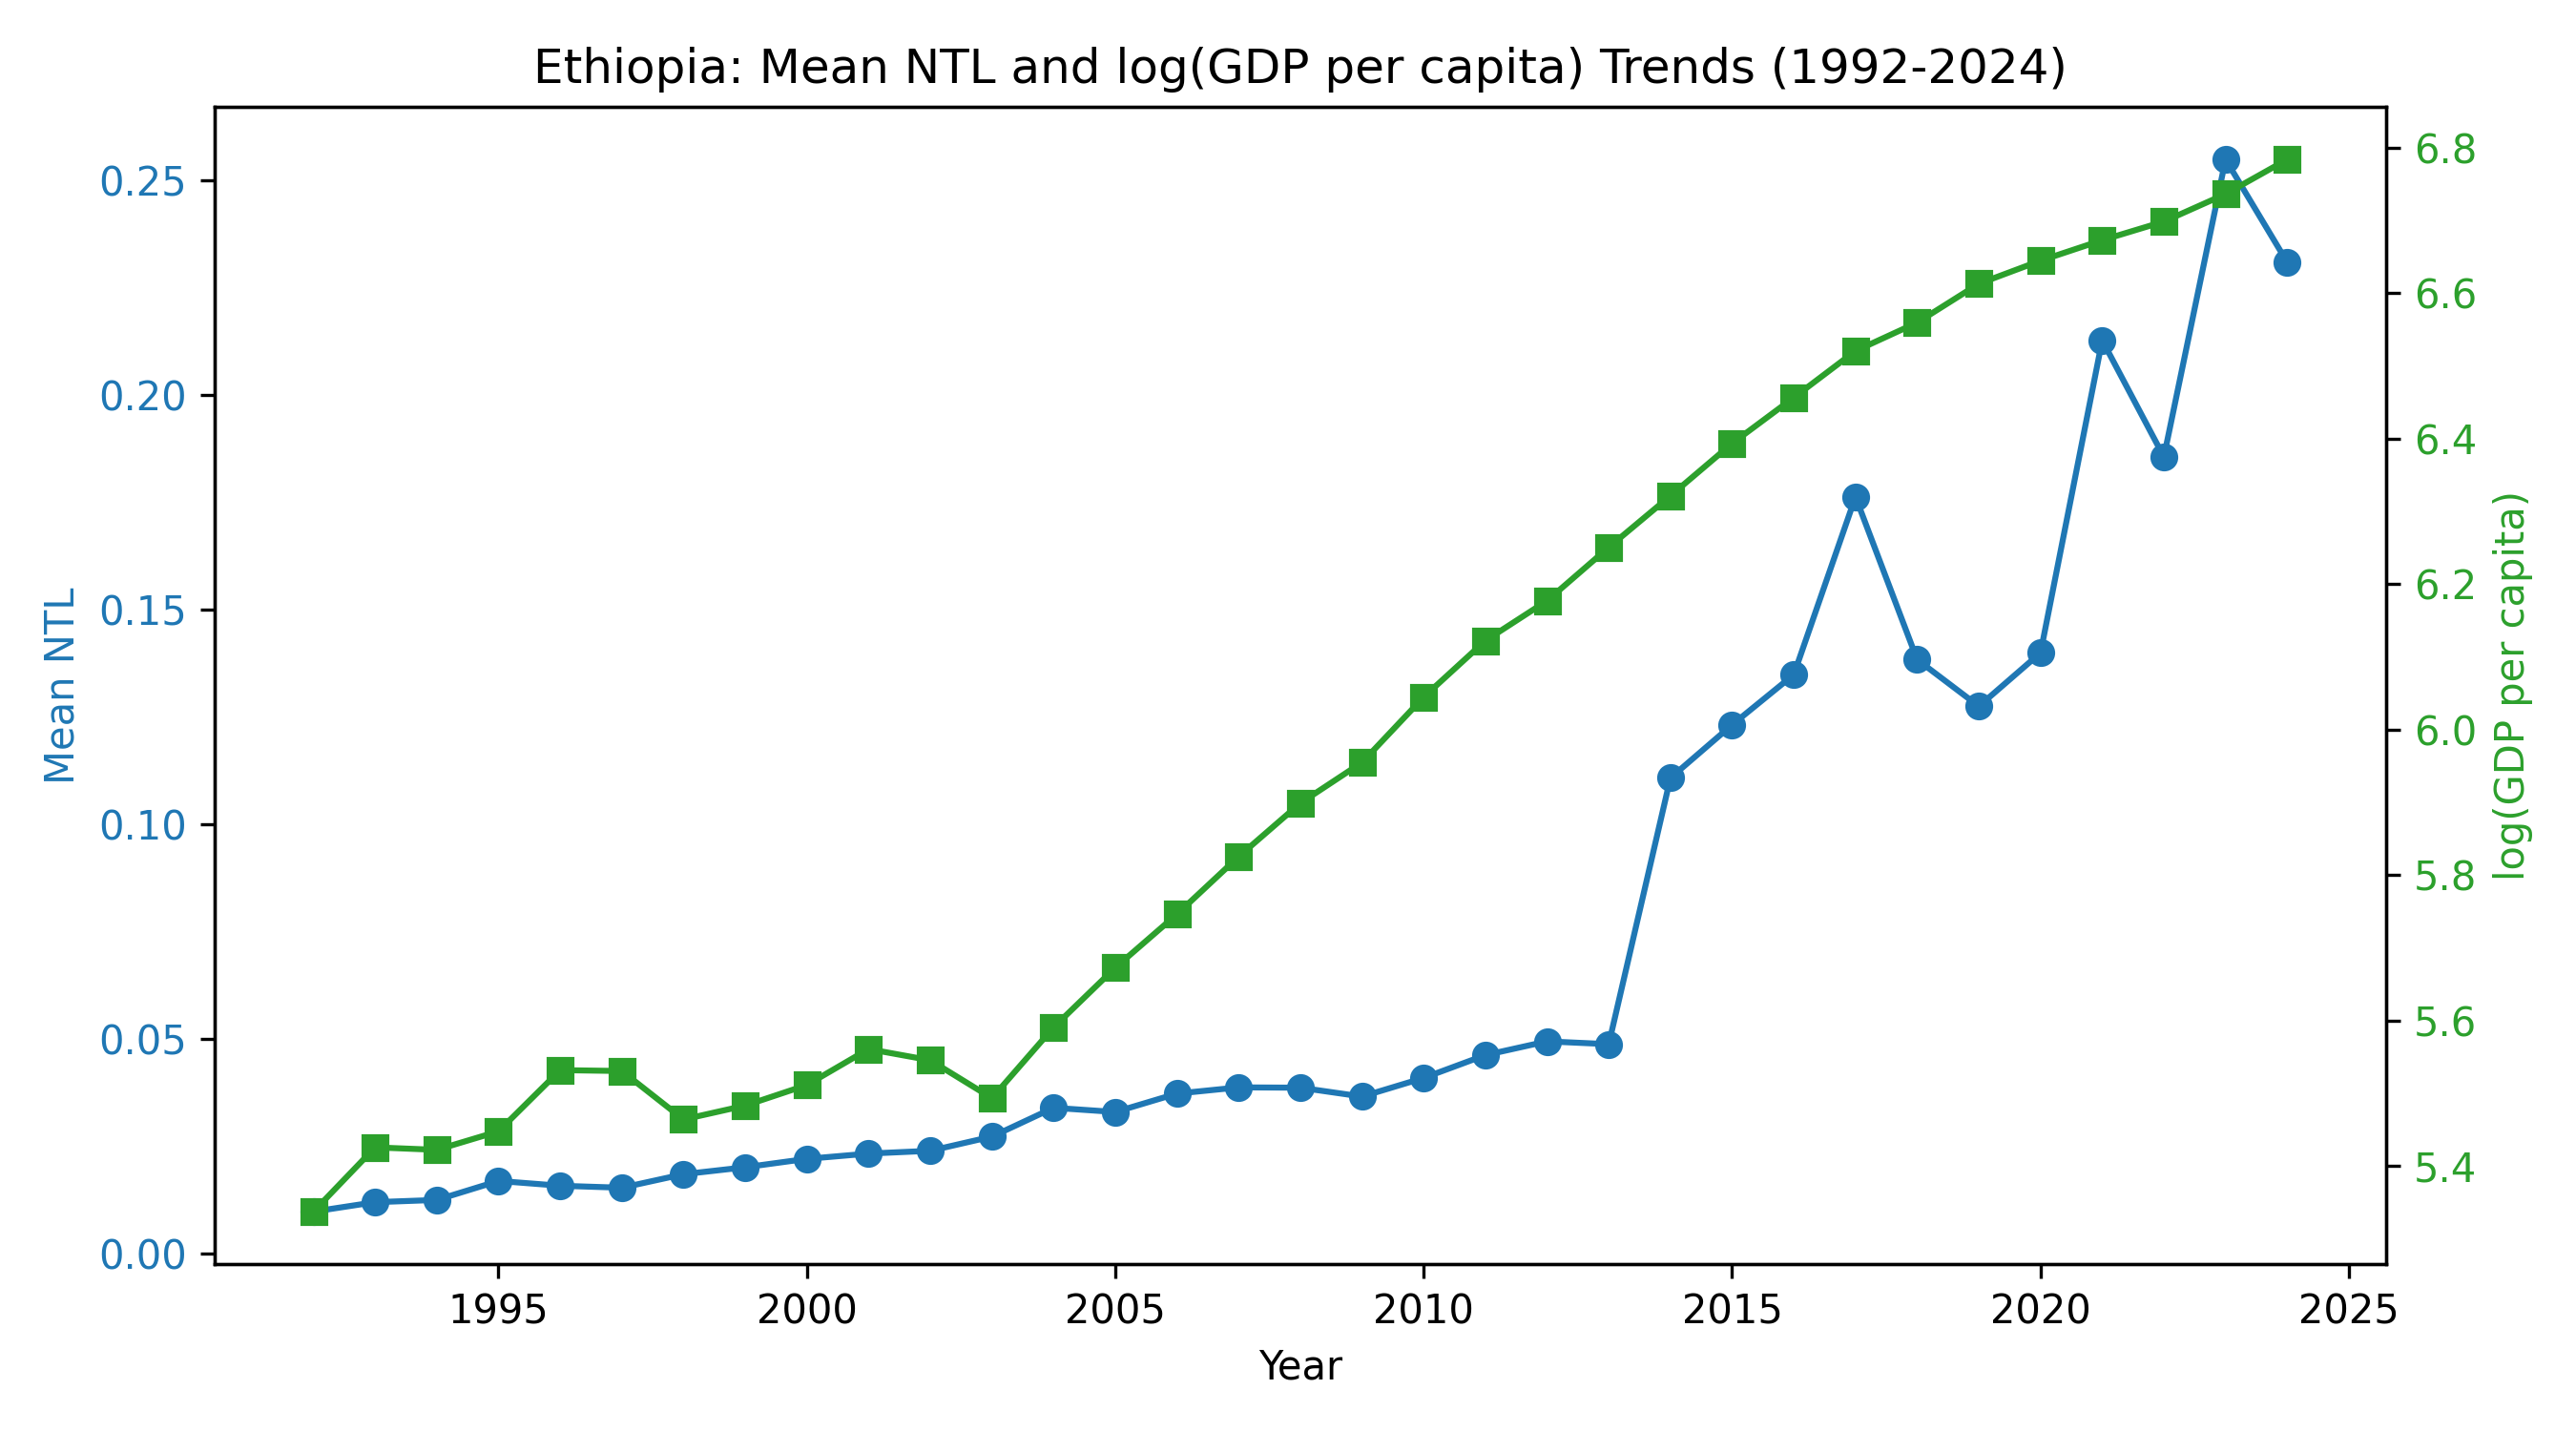
\includegraphics[width=0.7\textwidth]{../outputs/figures/national/ntl_gdp_combined_trend.png}
	\caption{Relationship between log(NTL) and log(GDP) at the national level.}
	\label{fig:ntl_gdp}
\end{figure}

\subsection{Regional Inequality}
Regional Gini coefficients are 0.715 in 1992, 0.513 in 2018, and 0.526 in 2024, indicating persistent but declining inequality across Ethiopia's regions.

\begin{figure}[ht]
	\centering
	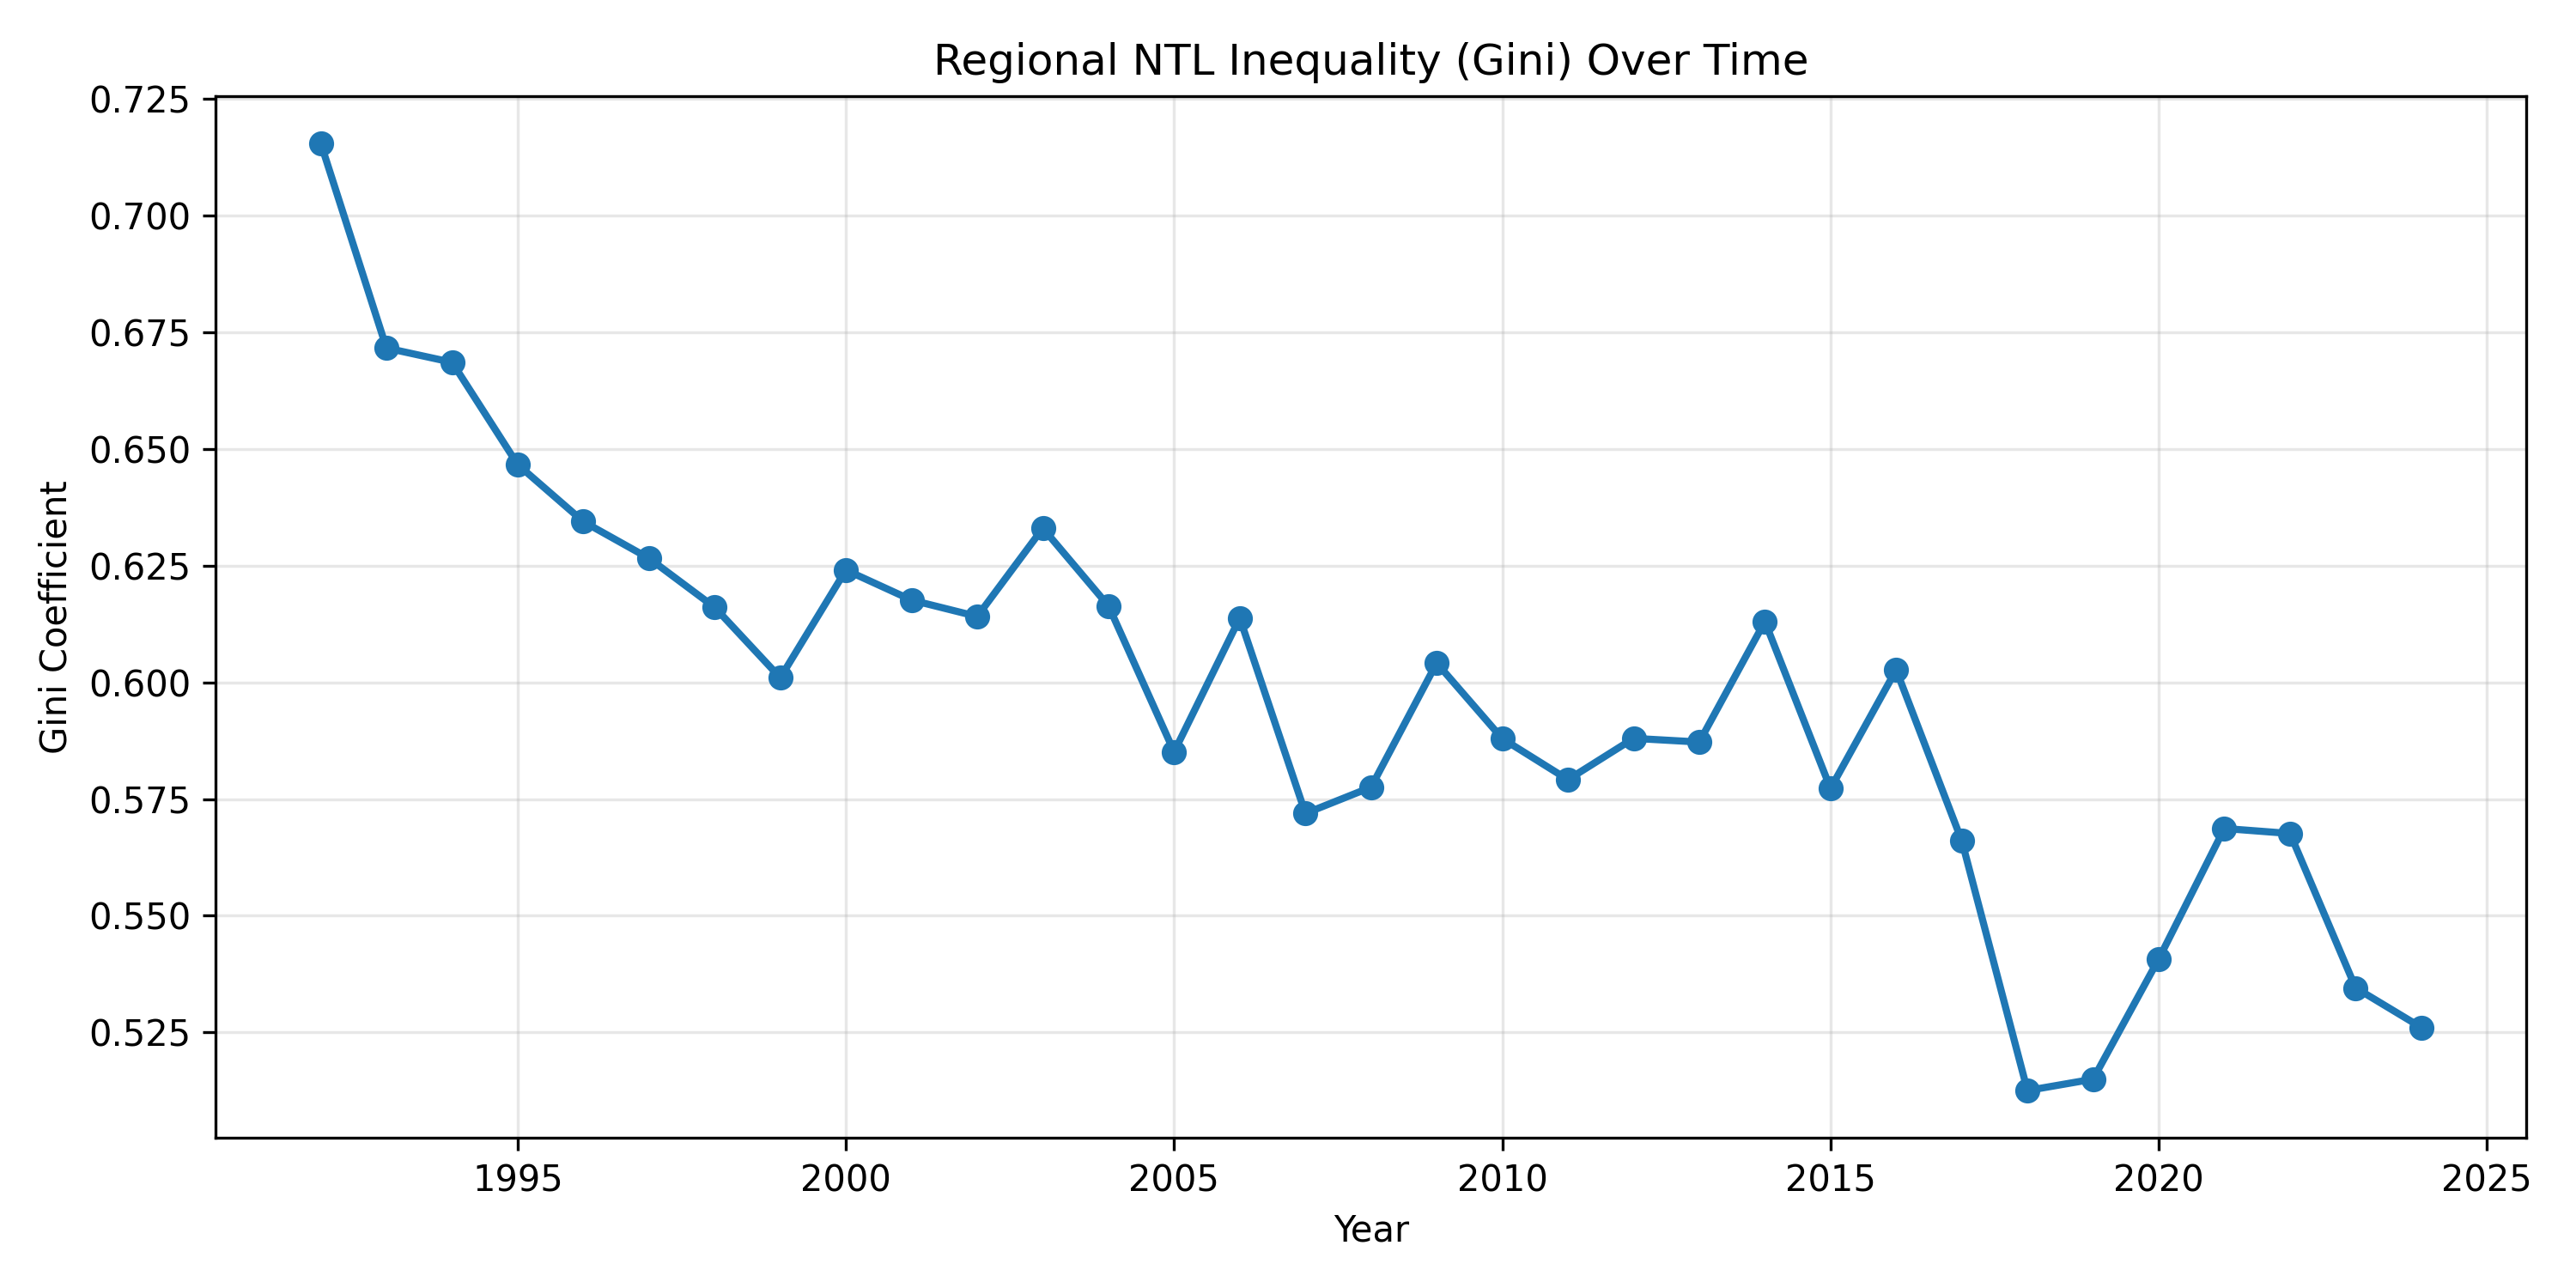
\includegraphics[width=0.7\textwidth]{../outputs/figures/regional/regional_ntl_gini_trend.png}
	\caption{Trends in regional NTL-based Gini coefficients, 1992--2024.}
	\label{fig:ntl_gini}
\end{figure}

\subsection{Regional NTL Trends}
\begin{figure}[ht]
	\centering
	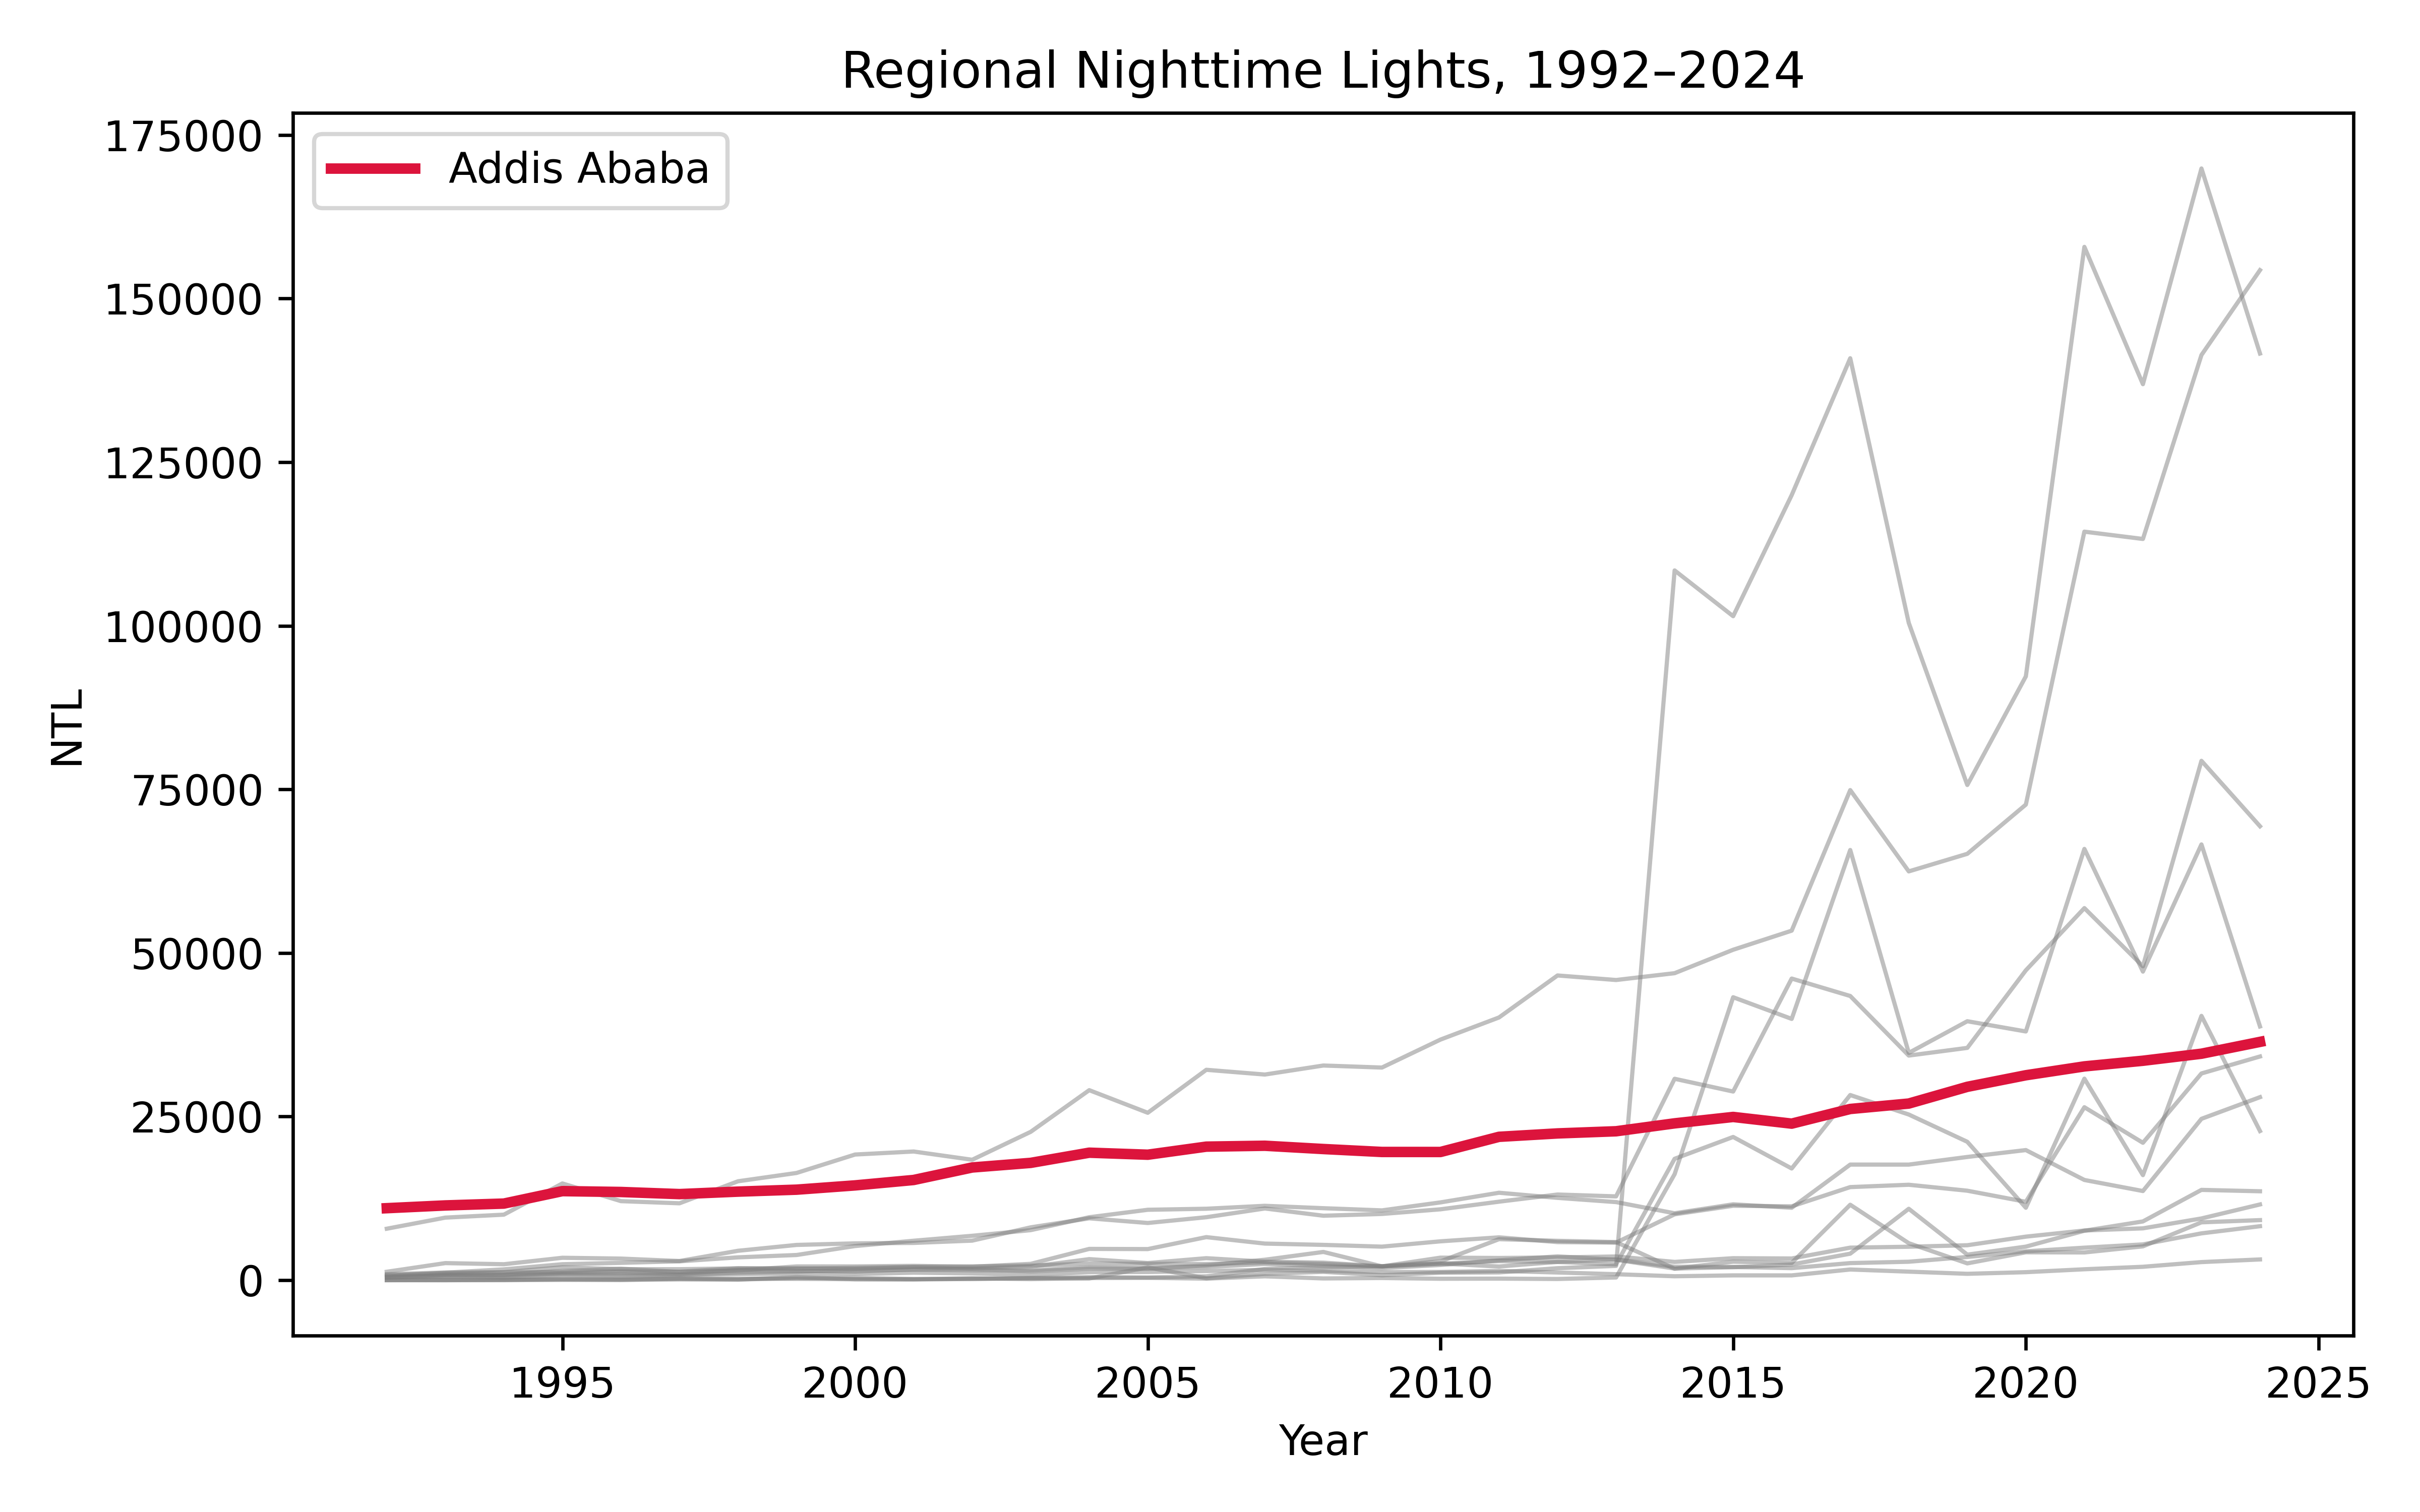
\includegraphics[width=0.7\textwidth]{../outputs/figures/regional/regional_luminosity_trends.png}
	\caption{Nighttime lights trends for all Ethiopian regions, 1992--2024.}
	\label{fig:ntl_trends}
\end{figure}

\subsection{Distribution of Nighttime Lights}
\begin{figure}[ht]
	\centering
	\includegraphics[width=0.7\textwidth]{../outputs/figures/regional/ntl_histogram.png}
	\caption{Distribution of regional nighttime lights (NTL) values, pooled across years.}
	\label{fig:ntl_hist}
\end{figure}

\subsection{Leader vs. Non-Leader Regions}
\begin{figure}[ht]
	\centering
	\includegraphics[width=0.7\textwidth]{../outputs/figures/regional/ntl_leader_vs_nonleader_trend.png}
	\caption{Mean NTL over time for leader and non-leader regions.}
	\label{fig:ntl_leader_trend}
\end{figure}

\begin{figure}[ht]
	\centering
	\includegraphics[width=0.7\textwidth]{../outputs/figures/regional/ntl_boxplot_by_leader.png}
	\caption{Distribution of NTL by leader status (boxplot, pooled years).}
	\label{fig:ntl_box_leader}
\end{figure}

\subsection{Leader Birth-Region Effects}


We estimate the effect of the lagged leader-region indicator (whether a region was the leader's birth region in the previous year) on log nighttime lights (lnNTL) using a range of panel regression models: pooled OLS, pooled OLS with entity effects, pooled OLS with time effects, within (entity + time fixed effects), between, and random effects. The results are summarized in Table~\ref{tab:leader_lag_regression_full}.

\begin{table}[ht]
\centering
\caption{Panel regression results: Lagged leader-region effect on lnNTL}
\label{tab:leader_lag_regression_full}
\begin{tabular}{lcccc}
\toprule
 & Pooled & Between & Random Effects & Fixed Effects \\
\midrule
\textbf{Leader\_region\_lag} & 1.09$^{***}$ & 1.38 & 0.97$^{***}$ & 0.46$^{**}$ \\
Std. Error & (0.20) & (0.98) & (0.23) & (0.20) \\
\textit{p}-value & 0.000 & 0.188 & 0.000 & 0.021 \\
\midrule
Entity Effects & No & No & Yes & Yes \\
Time Effects & No & No & No & Yes \\
Observations & 416 & 13 & 416 & 416 \\
R$^2$ & 0.030 & 0.053 & 0.022 & 0.009 \\
\bottomrule
\end{tabular}
\end{table}
\vspace{1mm}
\noindent\textit{Notes:} Dependent variable is lnNTL. All models use clustered standard errors. $^{***}$ $p<0.01$, $^{**}$ $p<0.05$. “Entity Effects” and “Time Effects” indicate inclusion of region and year fixed effects, respectively. Fixed Effects = entity and time FE; Random Effects = GLS random effects.

Across all panel regression models, the lagged leader-region indicator is positive, but only statistically significant in the pooled OLS, random effects, and fixed effects specifications. The largest effect is observed in the pooled OLS model ($\beta=1.09$, $p<0.001$), while the within (entity and time fixed effects) estimator, which best accounts for unobserved heterogeneity and time shocks, yields a smaller but still significant effect ($\beta=0.46$, $p=0.021$). The between estimator is positive but not statistically significant. However, the explanatory power of all models is low ($R^2 < 0.06$), and the estimated effect is sensitive to model specification. Thus, while there is some evidence of a lagged leader-region effect on regional luminosity, the result is not robust and should be interpreted with caution.

\subsection{Placebo and Event-Study Tests}

Placebo and event-study analyses do not yield significant results. The event study shows that all pre- and post-treatment coefficients are small, statistically insignificant, and confidence intervals include zero, indicating no evidence of significant pre-trends or treatment effects. This supports the absence of anticipation or omitted pre-treatment differences, but also suggests no detectable causal effect of leader-region status on NTL. The event-study design is further limited by the small number of transitions and treatment coding constraints, which restrict the strength of any causal interpretation.

\begin{figure}[ht]
	\centering
	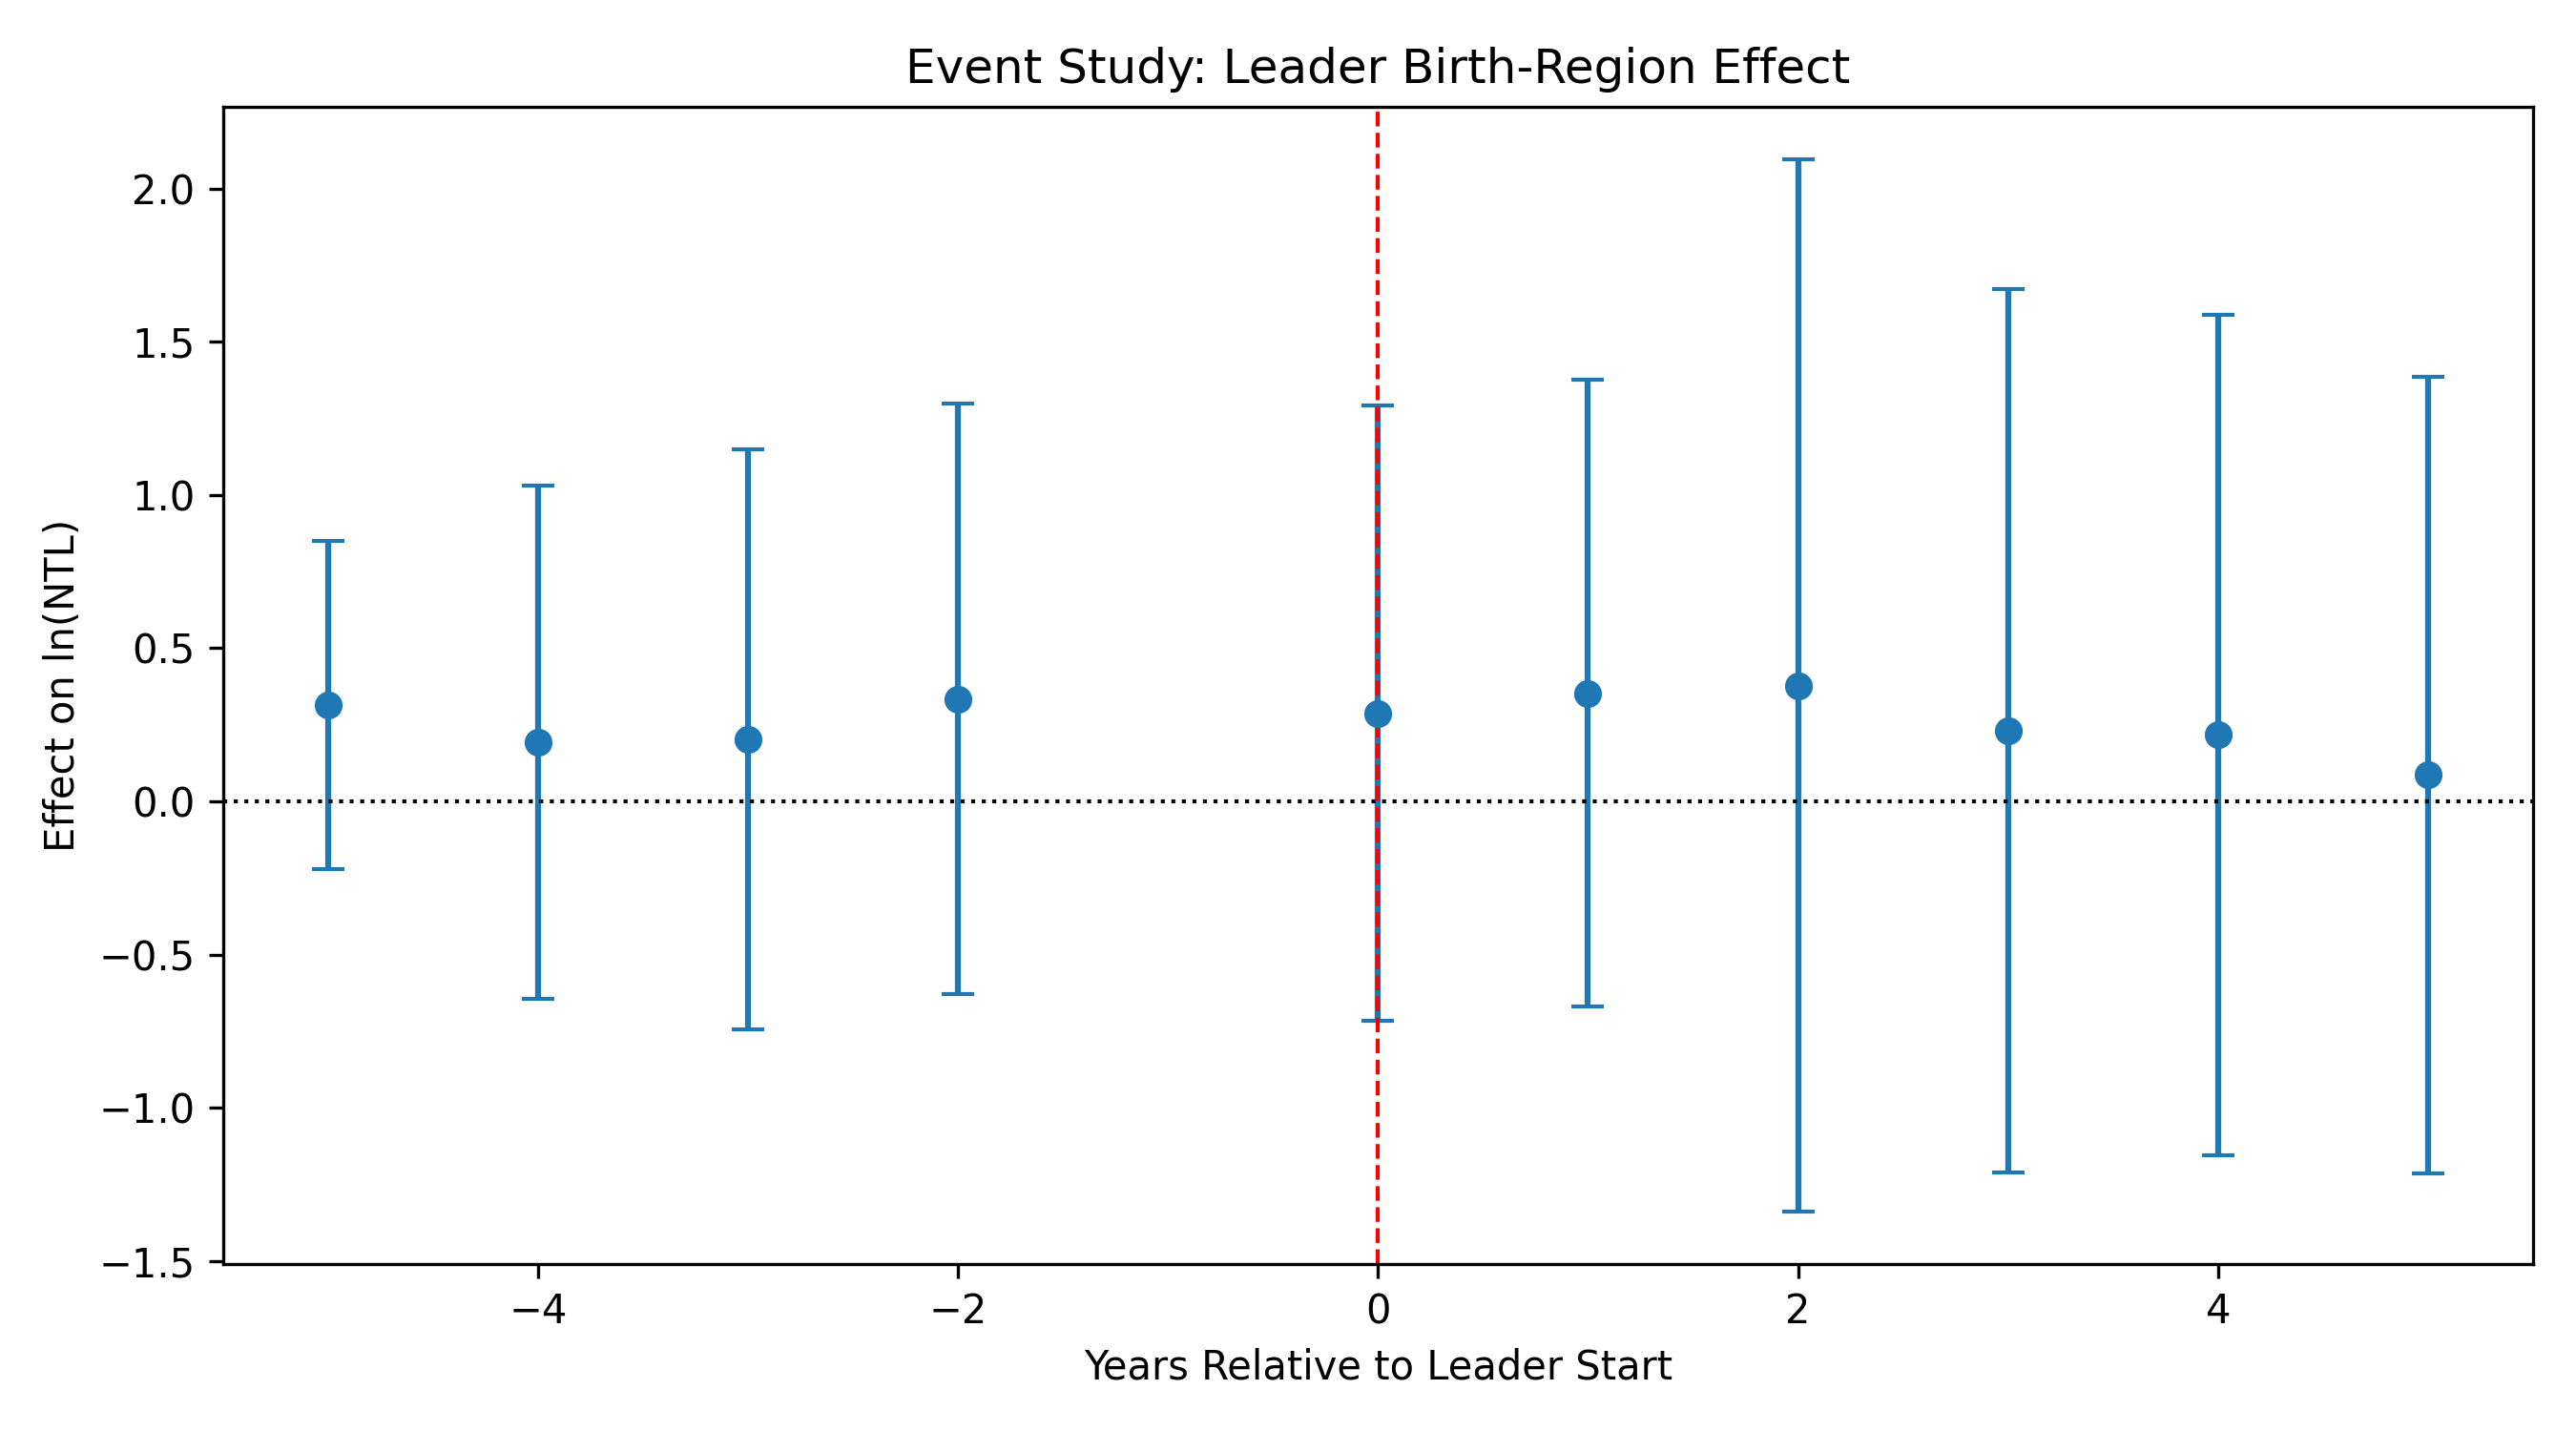
\includegraphics[width=0.7\textwidth]{../outputs/figures/regional/event_study_plot.png}
	\caption{Event-study analysis of leader-region effects. No significant pre-trends or treatment effects are detected.}
	\label{fig:event_study}
\end{figure}


\section{Robustness and Sensitivity}

Robustness and sensitivity checks reinforce the main findings. Including region-specific linear trends in the fixed effects model yields a positive but statistically insignificant leader-region effect (see Appendix). Using Driscoll--Kraay standard errors, the effect is positive and marginally significant in the full sample, but not robust to excluding special city-regions. Wild cluster bootstrap p-values are large ($p > 0.3$), indicating no robust evidence of favoritism. Varying the definition of leader regions and placebo tests (shifting treatment timing, shuffling region assignments) produce null or inconsistent effects (see Appendix). Taken together, these checks confirm that the main results are not sensitive to alternative specifications, coding choices, or random assignment. The evidence for regional favoritism remains weak and not robust across models.

% Uncomment and wrap in a figure environment if you want to include this simulation plot:
% \begin{figure}[ht]
%     \centering
%     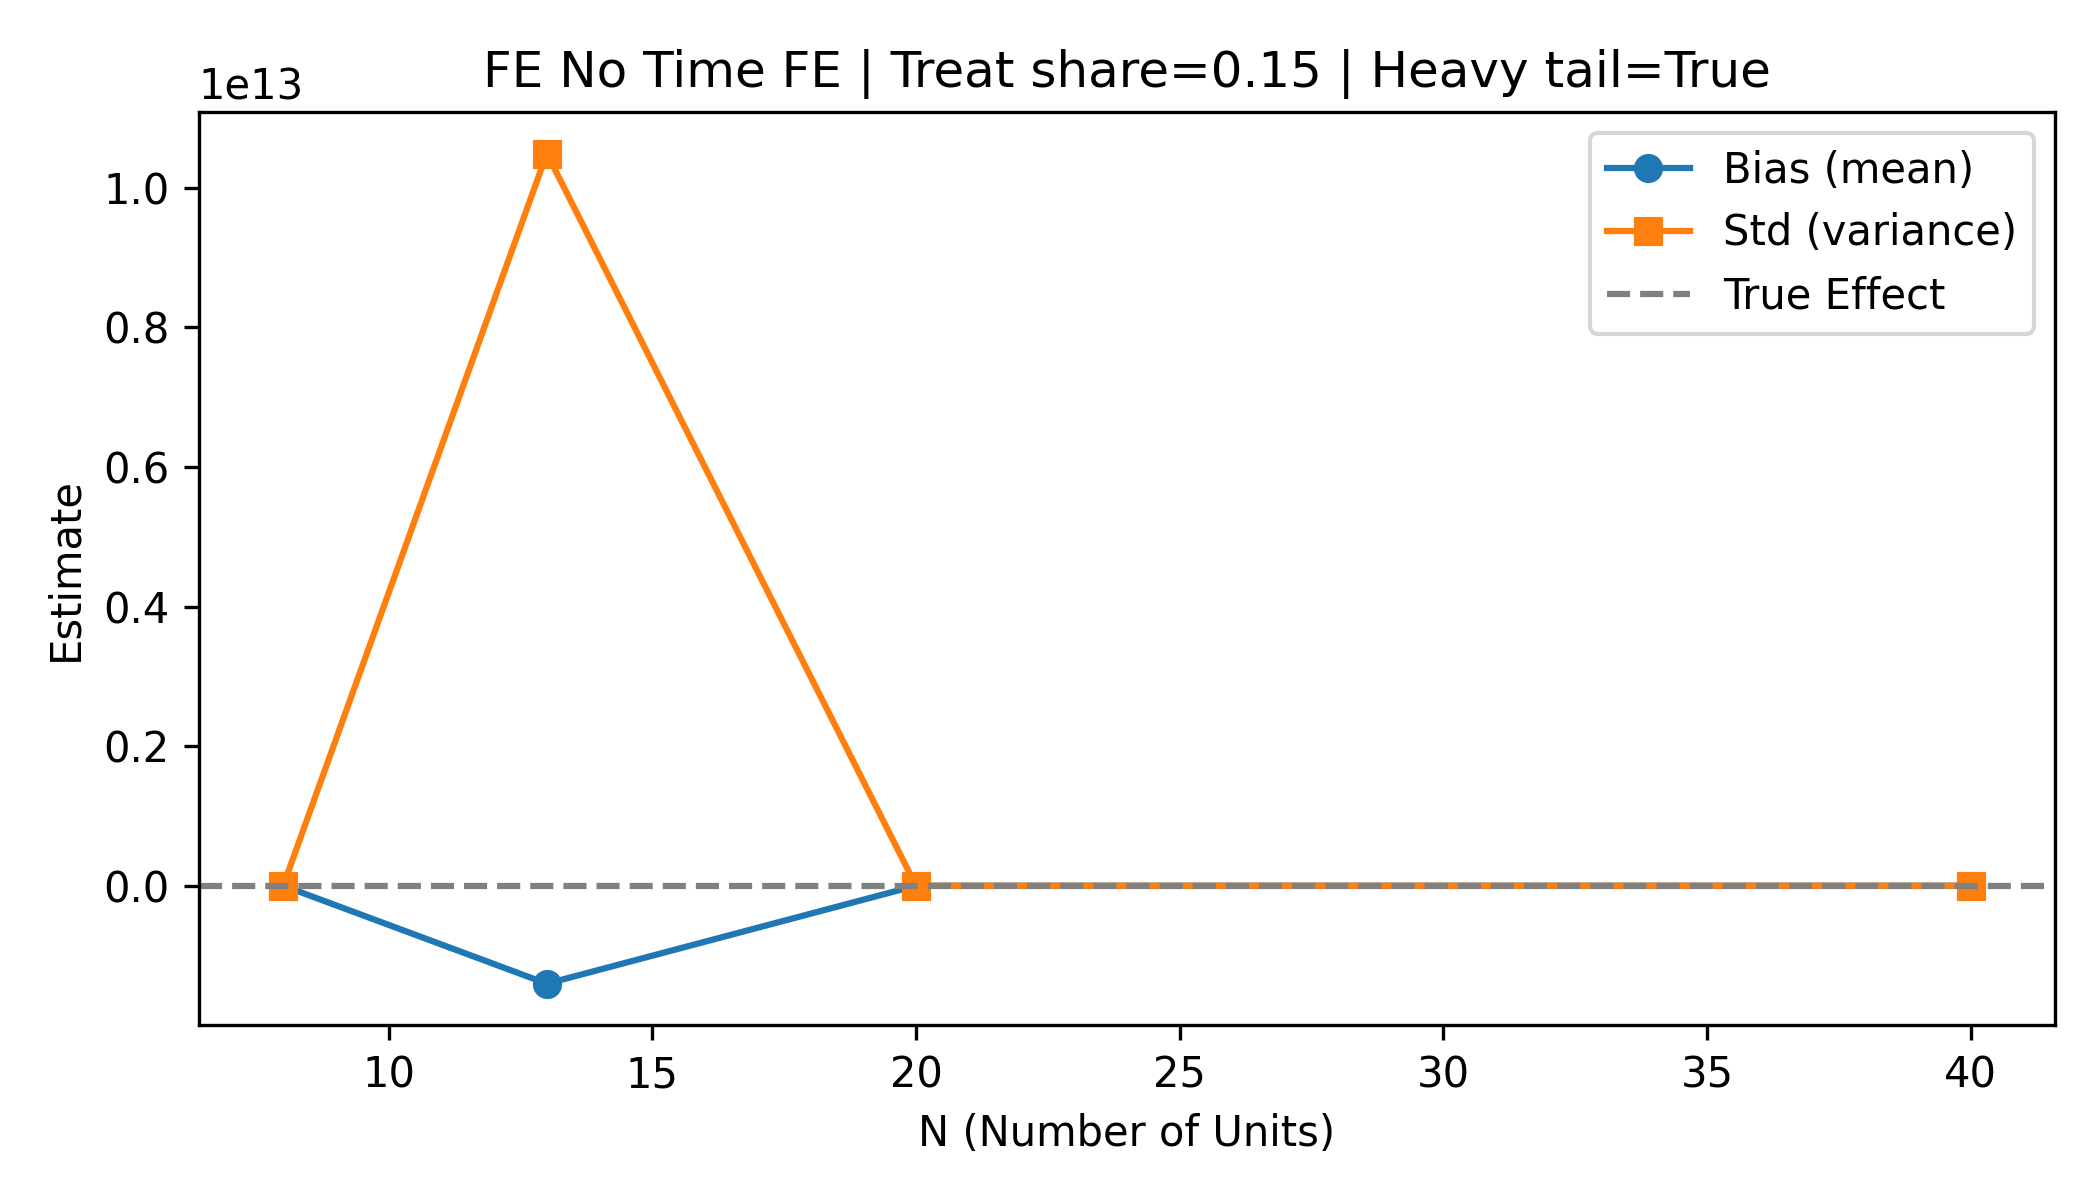
\includegraphics[width=0.7\textwidth]{../outputs/figures/simulation/sim_biasvar_N0.15_htTrue_feFalse.png}
%     \caption{Simulation of bias and variance in small-N panel settings with and without fixed effects.}
%     \label{fig:sim_biasvar}
% \end{figure}

\section{Discussion}

\section{Discussion}

This study contributes to the literature on political favoritism and regional inequality by providing a transparent, data-rich reassessment of the Ethiopian case. Our findings challenge the generalizability of cross-country evidence that leaders systematically favor their birth regions \citep{Hodler2014, BeiserMcGrath2021, Onana2024}. While prior work has documented strong links between political power and spatial allocation of resources, our results suggest that such mechanisms may be context-dependent and less pronounced in settings with centralized control, harmonized administrative boundaries, and limited regional autonomy \citep{Faguet2021, Wubneh2017}.

Mechanistically, the absence of robust leader-region effects in Ethiopia may reflect several factors. First, the highly centralized nature of fiscal and administrative authority under the EPRDF and its successors likely constrained the ability of national leaders to channel resources to their home regions, even if incentives for favoritism existed. Second, the harmonization of regional boundaries and the use of NTL as a proxy for economic activity may mask more localized or sector-specific favoritism that does not translate into broad-based regional growth. Third, the limited number of leader transitions and the high degree of collinearity between treatment and time effects reduce the statistical power to detect subtle favoritism, even if present.

These findings have important implications for external validity. The Ethiopian case demonstrates that the presence or absence of favoritism effects cannot be assumed to generalize across contexts, even within the same methodological framework. Studies in other countries with more frequent leadership turnover, greater regional autonomy, or less centralized control may yield different results. Moreover, the use of harmonized NTL data, while powerful for national and regional analysis, may not capture the full range of distributive politics, especially where favoritism operates through targeted projects, informal networks, or sub-regional channels \citep{Bluhm2022, Gibson2021}.

In interpreting these results, it is essential to move beyond simple correlations and consider the institutional and political mechanisms that shape distributive outcomes. The lack of detectable favoritism in Ethiopia does not imply the absence of political influence over resource allocation, but rather highlights the need for more granular data, richer identification strategies, and careful attention to context. Future research should explore alternative mechanisms—such as sectoral targeting, informal patronage, or coalition management—that may operate below the resolution of NTL-based measures.

\section{Limitations}

This study faces several important limitations that affect the strength and interpretation of its findings:

\begin{enumerate}
	\item \textbf{Small number of regions and leader transitions (most severe):} The limited sample size and infrequent changes in national leadership reduce statistical power and make it difficult to credibly identify causal effects. Most variation is cross-sectional, not within-region over time.
	\item \textbf{Potential endogeneity and lack of exogenous variation:} Assignment of leaders to regions is not random and may be correlated with unobserved factors affecting economic outcomes. Without valid instruments or natural experiments, causal claims are inherently weak.
	\item \textbf{Measurement error in NTL and GDP:} Nighttime lights are an imperfect proxy for economic activity, especially at the subnational level, and GDP data are sparse and potentially inconsistent across regions and years.
	\item \textbf{Event-study and pre-trend limitations:} The small number of treated units and transitions precludes robust pre-trend testing and limits the informativeness of event-study designs.
	\item \textbf{Administrative boundary harmonization and data construction:} Changes in regional boundaries and the need for harmonization may introduce aggregation bias or mask localized effects.
\end{enumerate}

Taken together, these limitations mean that the results should be interpreted as descriptive associations rather than definitive causal estimates. While panel methods and robustness checks mitigate some concerns, the evidence does not support strong causal claims about favoritism.

\section{Policy Implications}

The findings suggest that, in the Ethiopian context, there is no robust evidence of systematic favoritism toward leaders' birth regions as measured by regional nighttime lights and GDP. However, given the identification and data constraints, policymakers should avoid overinterpreting null results as proof of absence. Instead, the following policy implications are warranted:
\begin{itemize}
	\item \textbf{Invest in better data:} Improving the quality, frequency, and granularity of subnational economic data (including both NTL and official statistics) is essential for credible policy analysis and monitoring.
	\item \textbf{Support transparent and harmonized administrative boundaries:} Consistent regional definitions over time will improve the reliability of spatial analysis and reduce aggregation bias.
	\item \textbf{Interpret NTL-based evidence with caution:} Nighttime lights are a useful but imperfect proxy for economic activity, especially for detecting subtle or sector-specific favoritism. Complementary qualitative and administrative data should be used where possible.
	\item \textbf{Avoid strong claims about favoritism without stronger identification:} In small-N, high-leverage settings, robust causal inference is difficult. Policy conclusions should be tentative and emphasize the need for further research and richer data.
\end{itemize}

\section{Conclusion}
This study finds no strong empirical support for regional favoritism in Ethiopia using harmonized NTL and GDP data. The results emphasize the need for richer data, more exogenous variation, and careful diagnostics in future research on political favoritism and regional inequality.

\section{References}
% Bibliography will be generated automatically.
\bibliographystyle{plainnat}
\bibliography{references}

\section{Appendix}

\subsection*{Summary Statistics for Main Variables}
\begin{table}[ht]
\centering
\caption{Summary statistics for NTL, lnNTL, Mean\_NTL, and Leader\_region (regional panel, 1992--2024).}
\begin{tabular}{lcccccccc}
\toprule
Variable & Count & Mean & Std & Min & 25\% & 50\% & 75\% & Max \\
\midrule
NTL & 429 & 14167.6 & 25924.6 & 0.0 & 1306.0 & 3359.0 & 14484.0 & 169874.0 \\
lnNTL & 429 & 8.16 & 2.22 & -4.61 & 7.17 & 8.12 & 9.58 & 12.04 \\
Leader\_region & 429 & 0.11 & 0.32 & 0.0 & 0.0 & 0.0 & 0.0 & 1.0 \\
Mean\_NTL & 429 & 3.10 & 9.27 & 0.0 & 0.02 & 0.12 & 1.28 & 57.16 \\
\bottomrule
\end{tabular}
\label{tab:summary_stats}
\end{table}

\end{document}